\section{Introduction}

In this chapter will overview our proposed method and will further discuss prepossessing, analysing, post-processing and interference in our deep learning model. Later in this chapter we will discuss about our mixed datasets.

\section{Proposed Methodology}

In our proposed method we have used BottleneckCSP and SSP multiple times in the middle of the layers. For this, the model has been gone mush deep, and works well. Training process has slowed down due to these running in parallel, but the obtained model has accelerated. We have processed the data before feeding it to our modified core model. We have got better results using ORB and Hog combined. The model was able to easily objects due to the ORB making corners and edges distinguished. 





\subsection{Oriented FAST and Rotated BRIEF (ORB)}
Oriented FAST and Rotated BRIEF (ORB) performs as well as SIFT on the task of feature detection (and is better than SURF) while being almost two orders of magnitude faster. ORB builds on the well-known FAST key-point detector and the BRIEF descriptor. Both of these techniques are attractive because of their good performance and low cost \cite{orb}. ORB’s main contributions are as follows:

\begin{itemize}
    \item The addition of a fast and accurate orientation component to FAST
    \item The efficient computation of oriented BRIEF features
    \item Analysis of variance and correlation of oriented BRIEF features
    \item A learning method for de-correlating BRIEF features under rotational invariance, leading to better performance in nearest-neighbor applications
\end{itemize}


\begin{figure}[ht]
    \centering
    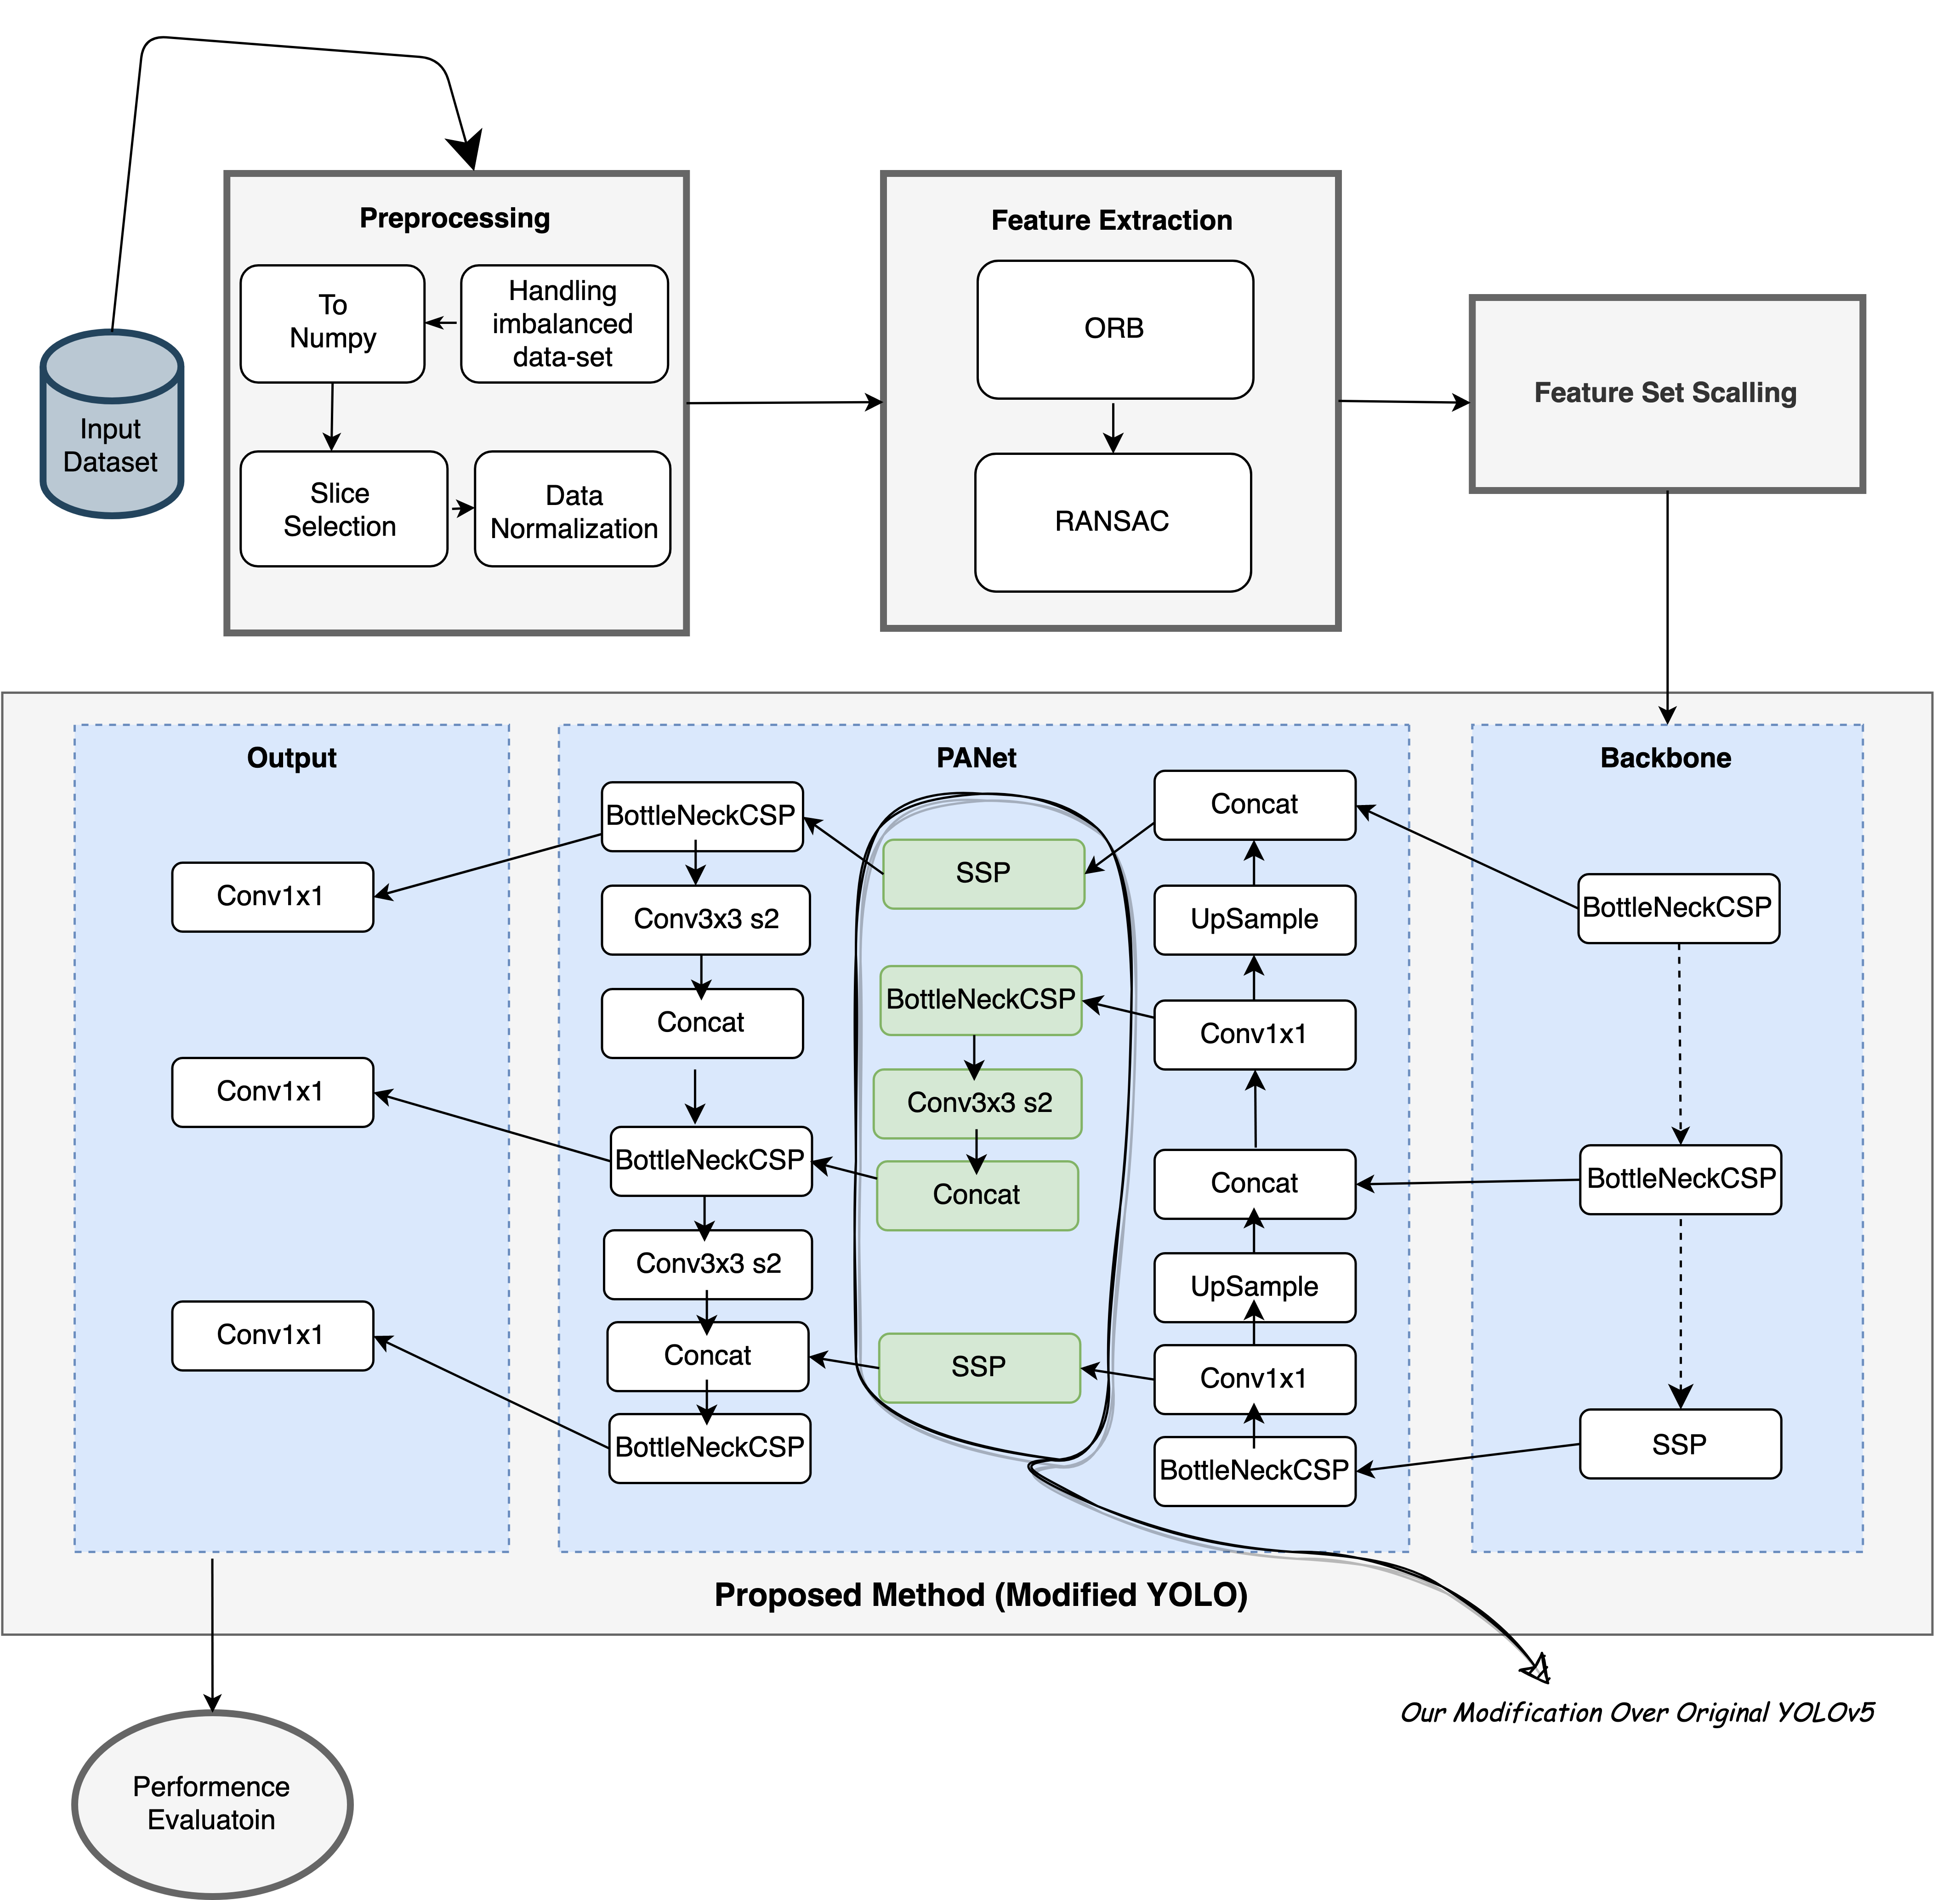
\includegraphics[max width=\textwidth]{images/ours/YOLO_M.drawio.png}
   \caption[Our Proposed Methodology]{Our Proposed Methodology: We have added some more layers in PANet}
    \label{fig:proposedmethodology}
\end{figure}


Features from accelerated segment test (FAST) is a corner detection method, which could be used to extract feature points and later used to track and map objects in many computer vision tasks. The FAST corner detector is very suitable for real-time video processing application because of this high-speed performance.

Brief (Binary robust independent elementary feature) start by smoothing image using a Gaussian kernel in order to prevent the descriptor from being sensitive to high-frequency noise.


\begin{table}
  \centering
  \caption[Modified YOLO Network Structure]{Modified YOLO Network Structure}
  \label{tab:yolo_network_mod}
    \begin{tabular}{p{0.1\textwidth} p{0.2\textwidth} p{0.3\textwidth} p{0.4\textwidth}}
      \toprule
        &     params & module                  &  arguments                     \\
     \hline
      0 &       8800 & Focus                   &  [3, 80, 3]                    \\
      1 &     115520 & Conv                    &  [80, 160, 3, 2]               \\
      2 &     315680 & BottleneckCSP           &  [160, 160, 4]                 \\
      3 &     461440 & Conv                    &  [160, 320, 3, 2]              \\
      4 &    3311680 & BottleneckCSP           &  [320, 320, 12]                \\
      5 &    1844480 & Conv                    &  [320, 640, 3, 2]              \\
      6 &   13228160 & BottleneckCSP           &  [640, 640, 12]                \\
      7 &    7375360 & Conv                    &  [640, 1280, 3, 2]             \\
      8 &    4099840 & SPP                     &  [1280, 1280, [5, 9, 13]]      \\
      9 &   20087040 & BottleneckCSP           &  [1280, 1280, 4, False]        \\
     10 &     820480 & Conv                    &  [1280, 640, 1, 1]             \\
     11 &          0 & Upsample                &  [None, 2, 'nearest']          \\
     12 &          0 & Concat                  &  [1]                           \\
     13 &    5435520 & BottleneckCSP           &  [1280, 640, 4, False]         \\
     14 &     205440 & Conv                    &  [640, 320, 1, 1]              \\
     15 &          0 & Upsample                &  [None, 2, 'nearest']          \\
     16 &          0 & Concat                  &  [1]                           \\
     17 &    1360960 & BottleneckCSP           &  [640, 320, 4, False]          \\
     18 &     922240 & Conv                    &  [320, 320, 3, 2]              \\
     19 &          0 & Concat                  &  [1]                           \\
     20 &    5025920 & BottleneckCSP           &  [640, 640, 4, False]          \\
     21 &    3687680 & Conv                    &  [640, 640, 3, 2]              \\
     22 &          0 & Concat                  &  [1]                           \\
     23 &   20087040 & BottleneckCSP           &  [1280, 1280, 4, False]        \\
     24 &     174954 & Detect                  &  [21, [[0, 1, 2, 3, 4, 5], [0, 1, 2, 3, 4, 5], [0, 1, 2, 3, 4, 5]], [320, 640, 1280]] \\

\bottomrule
    \end{tabular}
  
\end{table}



\subsection{RANdom SAmple Consensus (RANSAC)}
These descriptors between image pairs are then matched against each other to identify the best match with the minimum distance by brute force method. As the matches often contain outliers, a consistency check such as RANSAC is often used to remove inconsistent matches.~\ref{fig:ransac} shows the match points of an input image pair after adopting the RANSAC algorithm. The consistent matches are then used to model a transformation matrix for estimating a global motion for every pixel \cite{10.1145/358669.358692}.

\begin{figure}[ht]
    \centering
    \includegraphics[max width=\textwidth]{images/ours/ransac.png}
   \caption[ORB and RANSAC Preview]{The match points of an input image pair before and after adopting RANSAC algorithm. (a) initial match, (b) filtered match points.}
    \label{fig:ransac}
\end{figure}


\subsection{BottleneckCSP}
A Bottleneck Residual Block is a variant of the residual block that utilises 1x1 convolutions to create a bottleneck. The use of a bottleneck reduces the number of parameters and matrix multiplications. The idea is to make residual blocks as thin as possible to increase depth and have less parameters \cite{wang2019cspnet}. They were introduced as part of the ResNet architecture, and are used as part of deeper ResNets such as ResNet-50 and ResNet-101.


\subsection{Spatial Pyramid Pooling (SPP)}
 Spatial Pyramid Pooling (SPP) is a pooling layer that removes the fixed-size constraint of the network, i.e. a CNN does not require a fixed-size input image. Specifically, we add an SPP layer on top of the last convolutional layer. The SPP layer pools the features and generates fixed-length outputs, which are then fed into the fully-connected layers (or other classifiers) \cite{10.1007/978-3-319-10578-9_23}. In other words, we perform some information aggregation at a deeper stage of the network hierarchy (between convolutional layers and fully-connected layers) to avoid the need for cropping or warping at the beginning.
\newpage

%\section{Other discussion}


\section{Dataset Analysis}
Our new dataset has 100000 cropped images after discarding some of the images which only containing background. Of these, 10000 contain 30000 vehicles in total. Although our source images cover much of Bangladesh and India, an imbalance still exists between different classes of vehicles in our benchmark. This is unavoidable: classes such as auto rickshaw. It can be from different viewpoints, have different ground sampling distances (gsd), different image sizes, aspect ratios, color, etc. Vehicles in different data may be significantly different in size and appearance.~\ref{fig:dataset_collage} shows different images from four different datasets. It is obvious how different the VOC data is from any of the elevated data, while the VEDAI and AFVID data are somewhat similar, and the AF Building Camera data is more similar to the aerial and satellite data. To change the number of classes used, more than just the classes setting will need to be changed; the number of filters in the last convolutional layer must be altered to reflect the changed number of classes. The number of filters is set by $num(classes + coords + 1)$, where num is number of anchor boxes, and coords is four corresponding to the four coordinates used to define a bounding box.

\begin{figure}[ht]
    \centering
    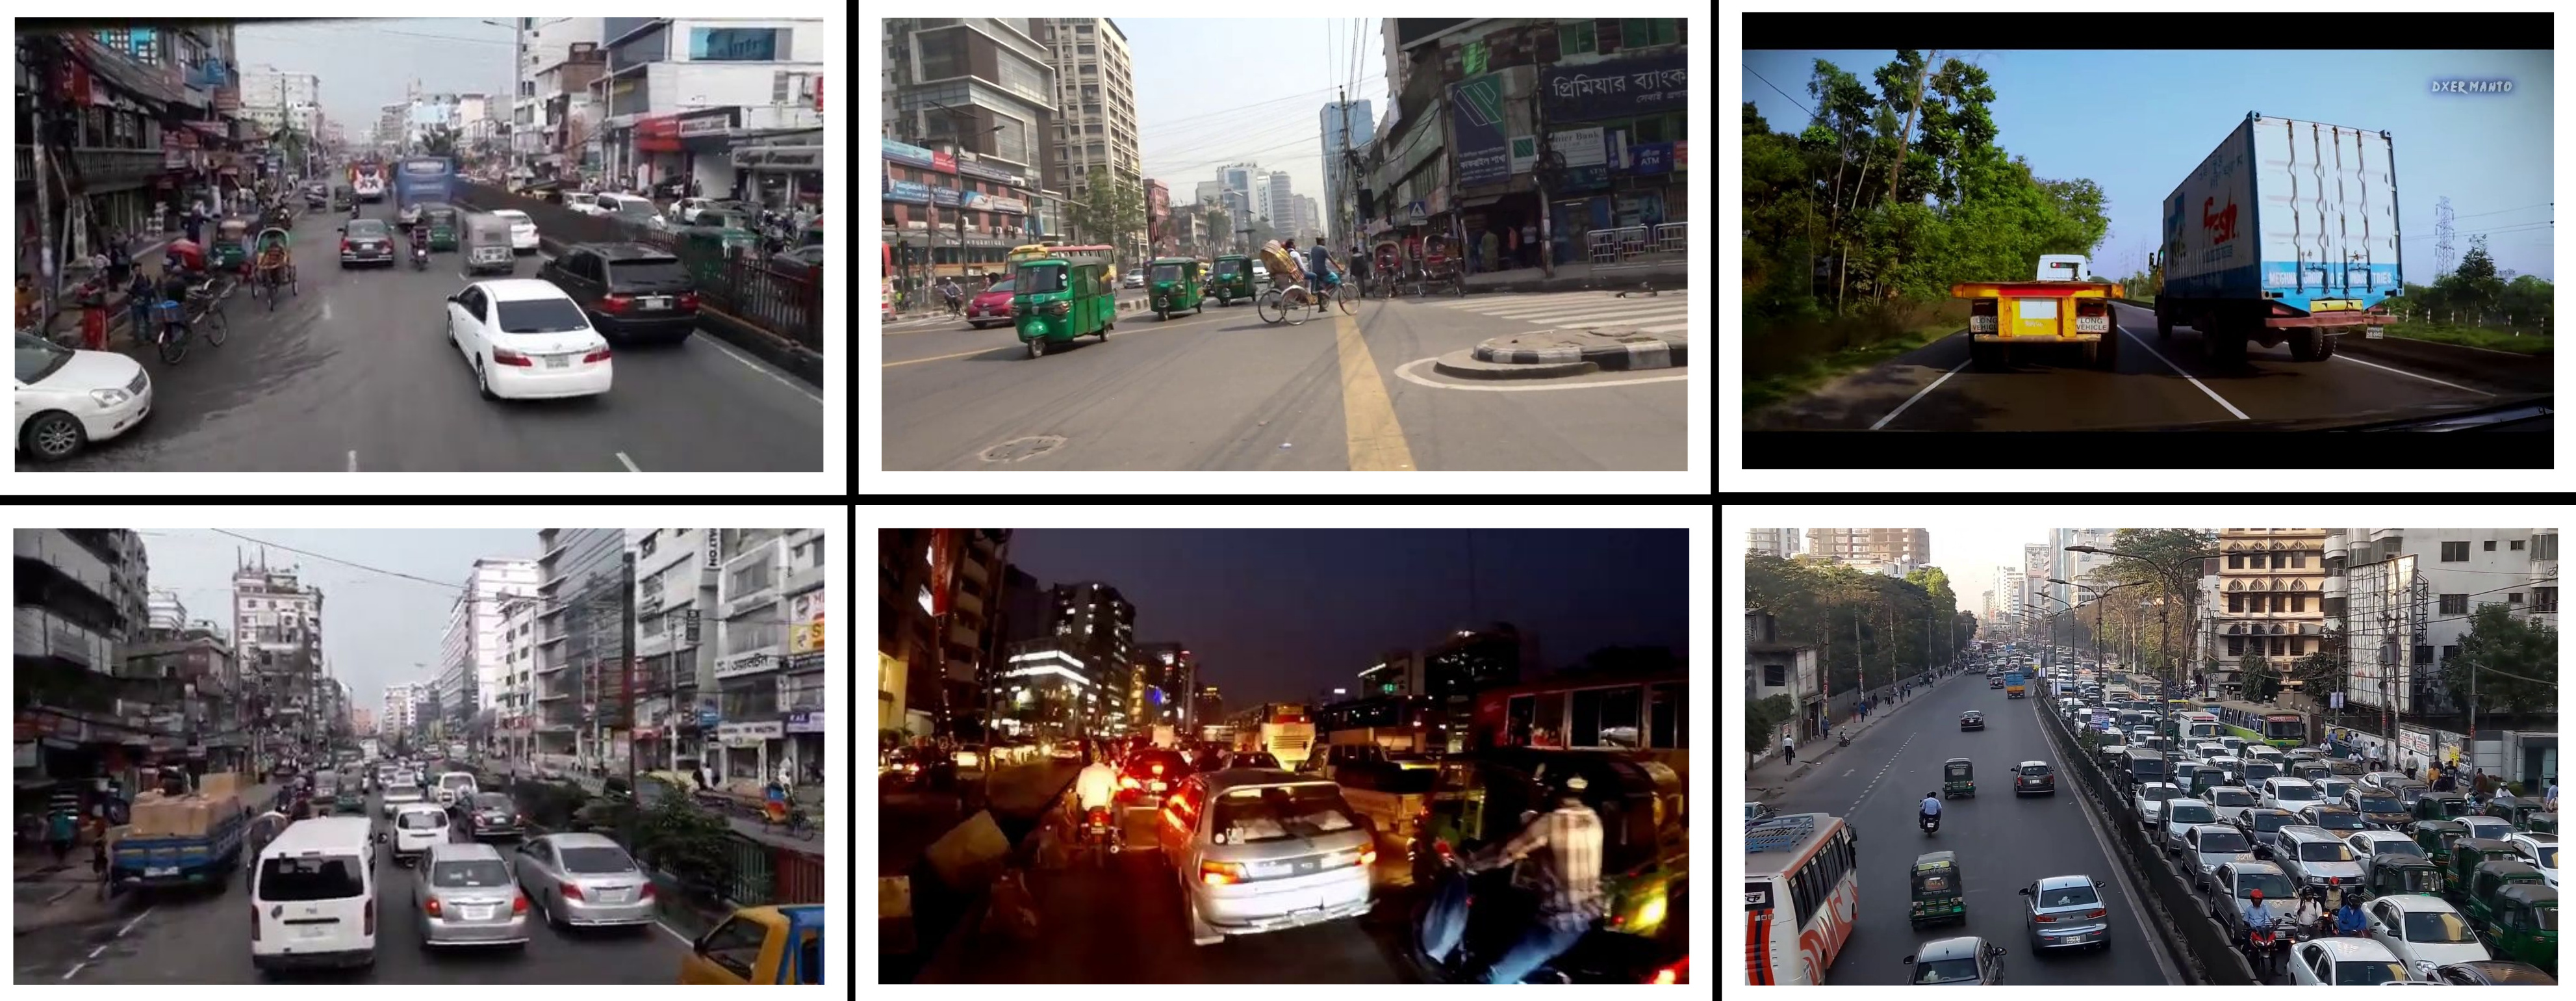
\includegraphics[max width=\textwidth]{images/ours/dataset-collage.jpg}
   \caption[Sample Data From Dhaka AI Dataset]{  Some sample data from Dhaka AI dataset }
    \label{fig:dataset_collage}
\end{figure}

\subsection{COCO Dataset Details}

\begin{figure}[ht]
    \centering
    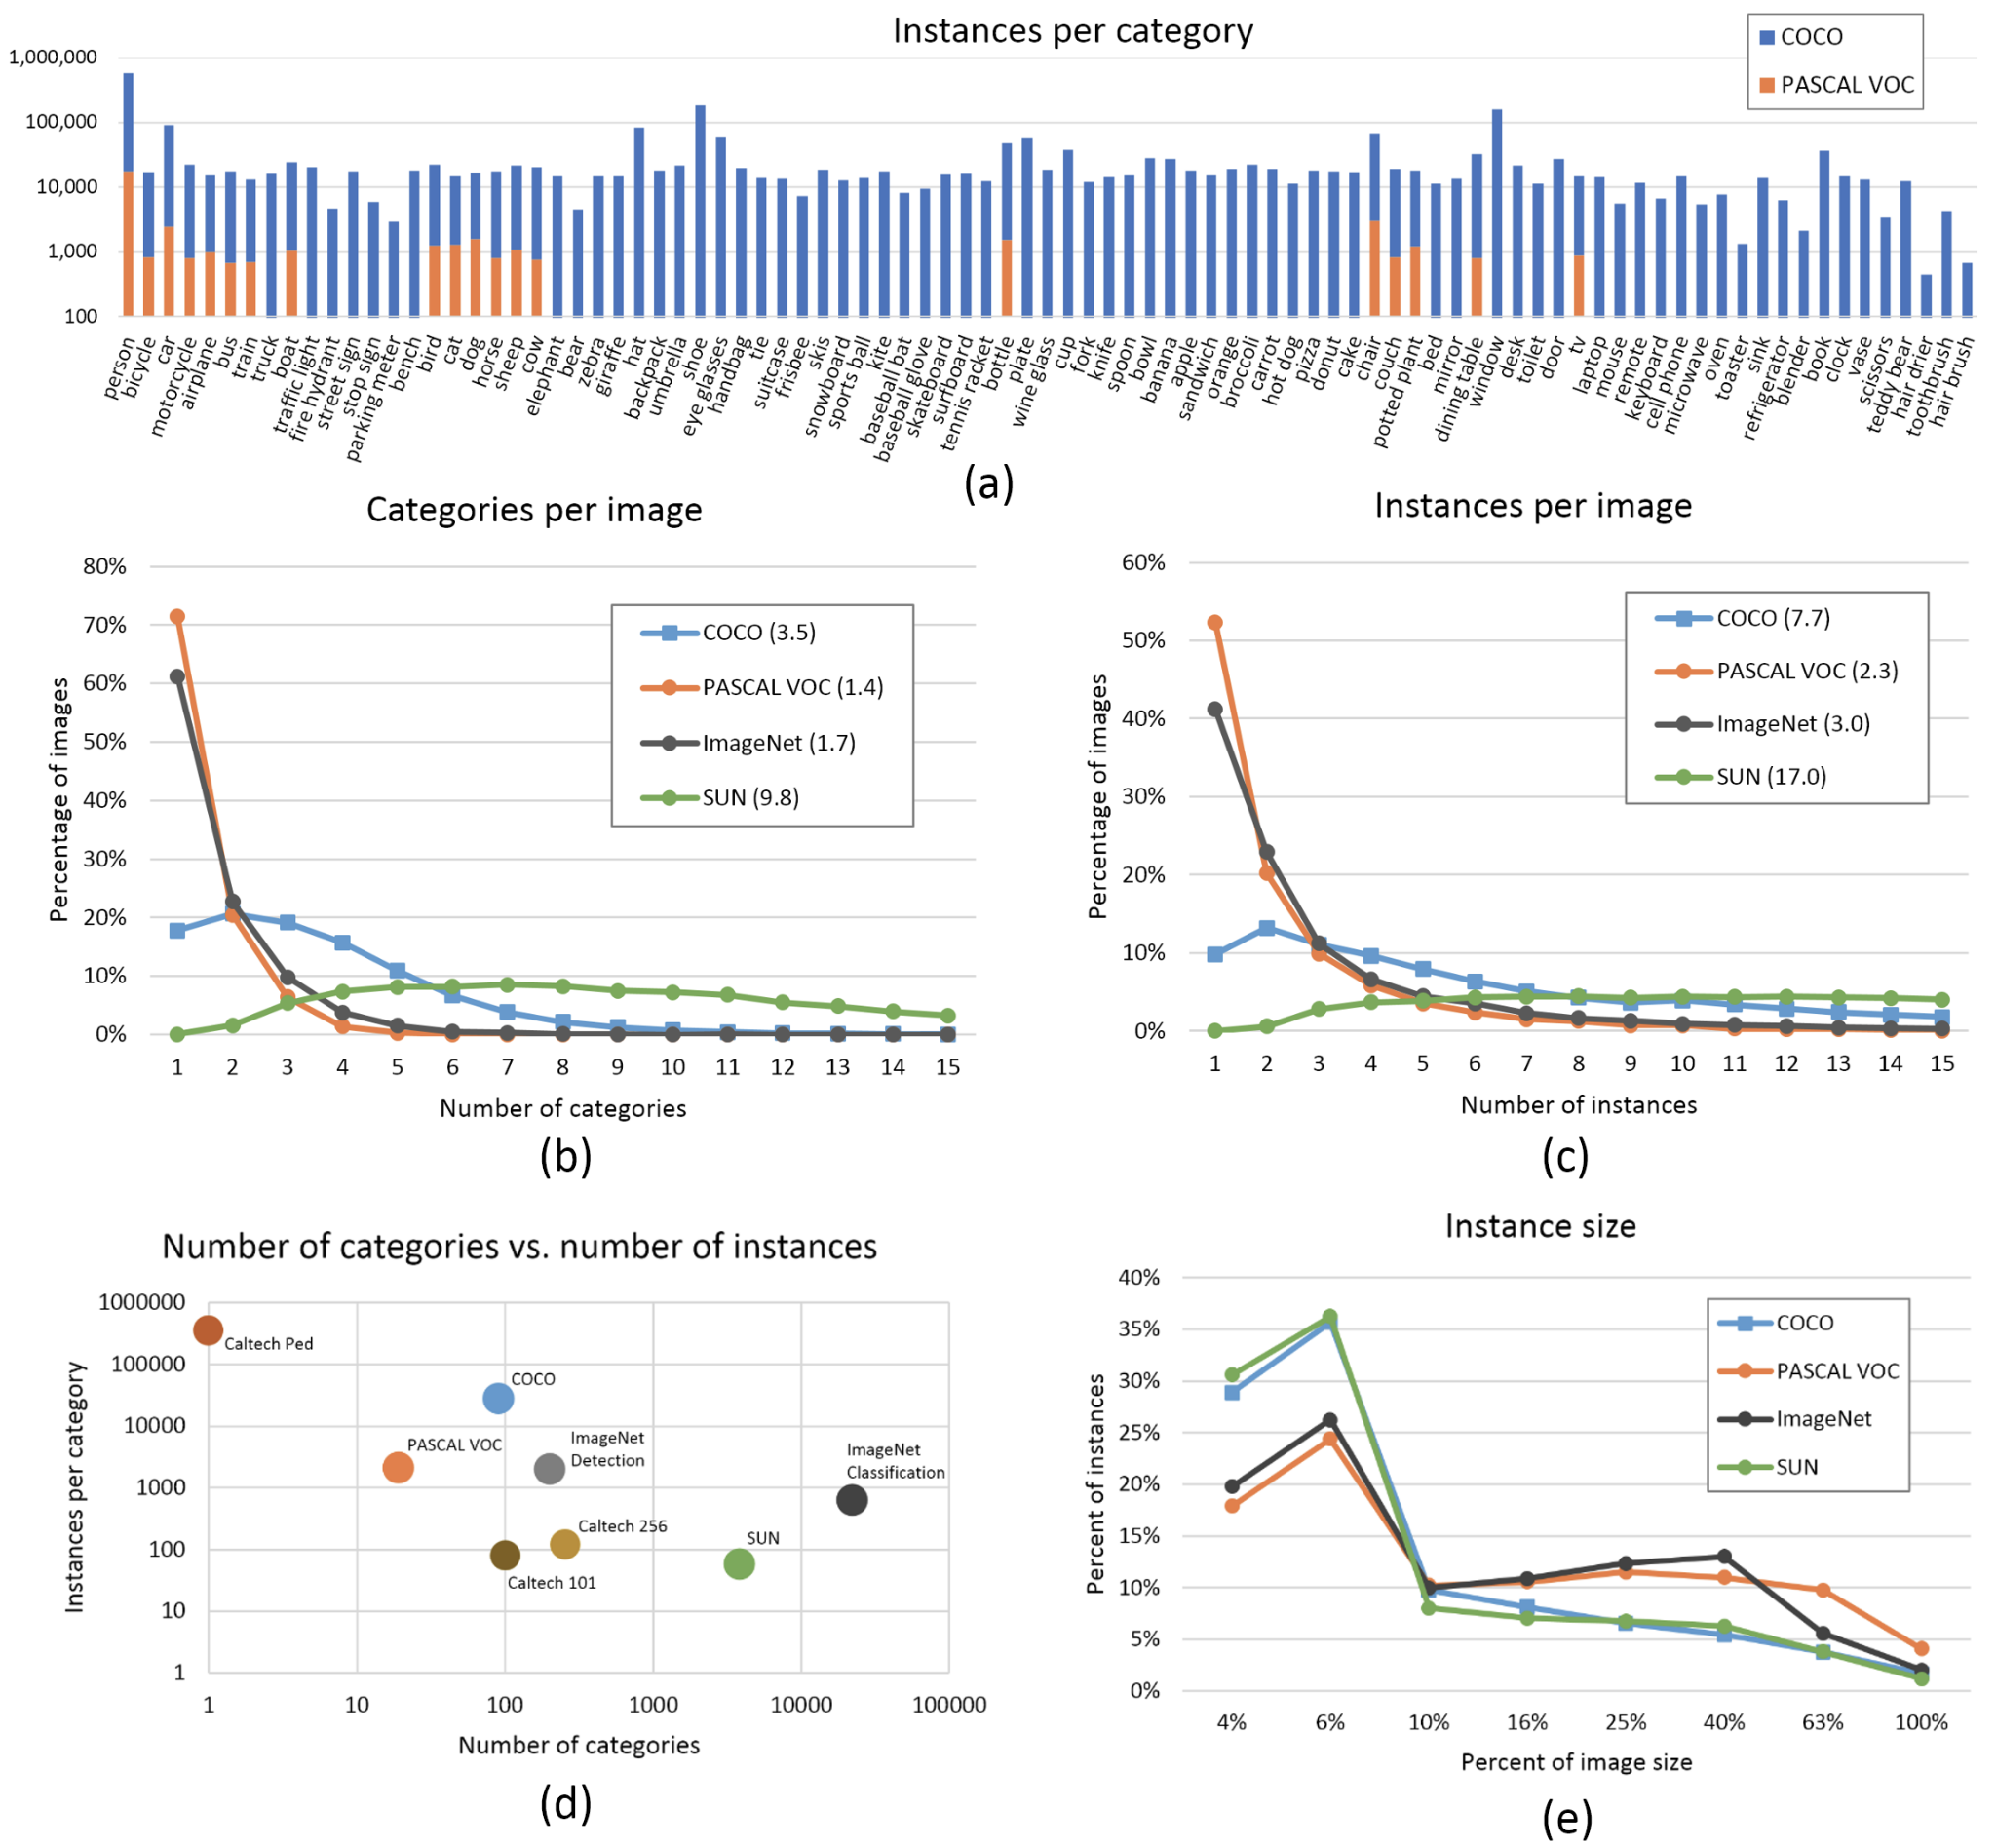
\includegraphics[max width=\textwidth]{images/ours/coco-details.png}
   \caption[COCO Dataset Details]{COCO dataset details \cite{lin2015microsoft}}
    \label{fig:coco_details}
\end{figure}

\begin{itemize}
  \item \textbf{Images per class} 1500 images per class recommended
  \item \textbf{Instances per class} 10000 instances (labeled objects) per class recommended
  \item \textbf{Image variety} Must be representative of deployed environment. For real-world use cases we recommend images from different times of day, different seasons, different weather, different lighting, different angles, different sources (scraped online, collected locally, different cameras) etc.
 \item \textbf{Label consistency} All instances of all classes in all images must be labelled. Partial labelling will not work.
 \item \textbf{Label accuracy} Labels must closely enclose each object. No space should exist between an object and it's bounding box. No objects should be missing a label.
 \item \textbf{Background images} Background images are images with no objects that are added to a dataset to reduce False Positives (FP). We recommend about 0-10\% background images to help reduce FPs (COCO has 1000 background images for reference, 1\% of the total). No labels are required for background images.
\end{itemize}



~\ref{fig:coco_details} is showing details of COCO dataset. We used pretrained model trained by COCO dataset then fitted our model with our dataset as needed. This helps to reduce time to train model efficiently. We used COCO dataset in every model.

\subsection{Dhaka AI Dataset}
We have used  a mixed dataset from Indian Driving Dataset and Dhaka AI Traffic Detection Challenge Dataset.

\begin{figure}[ht]
    \centering
    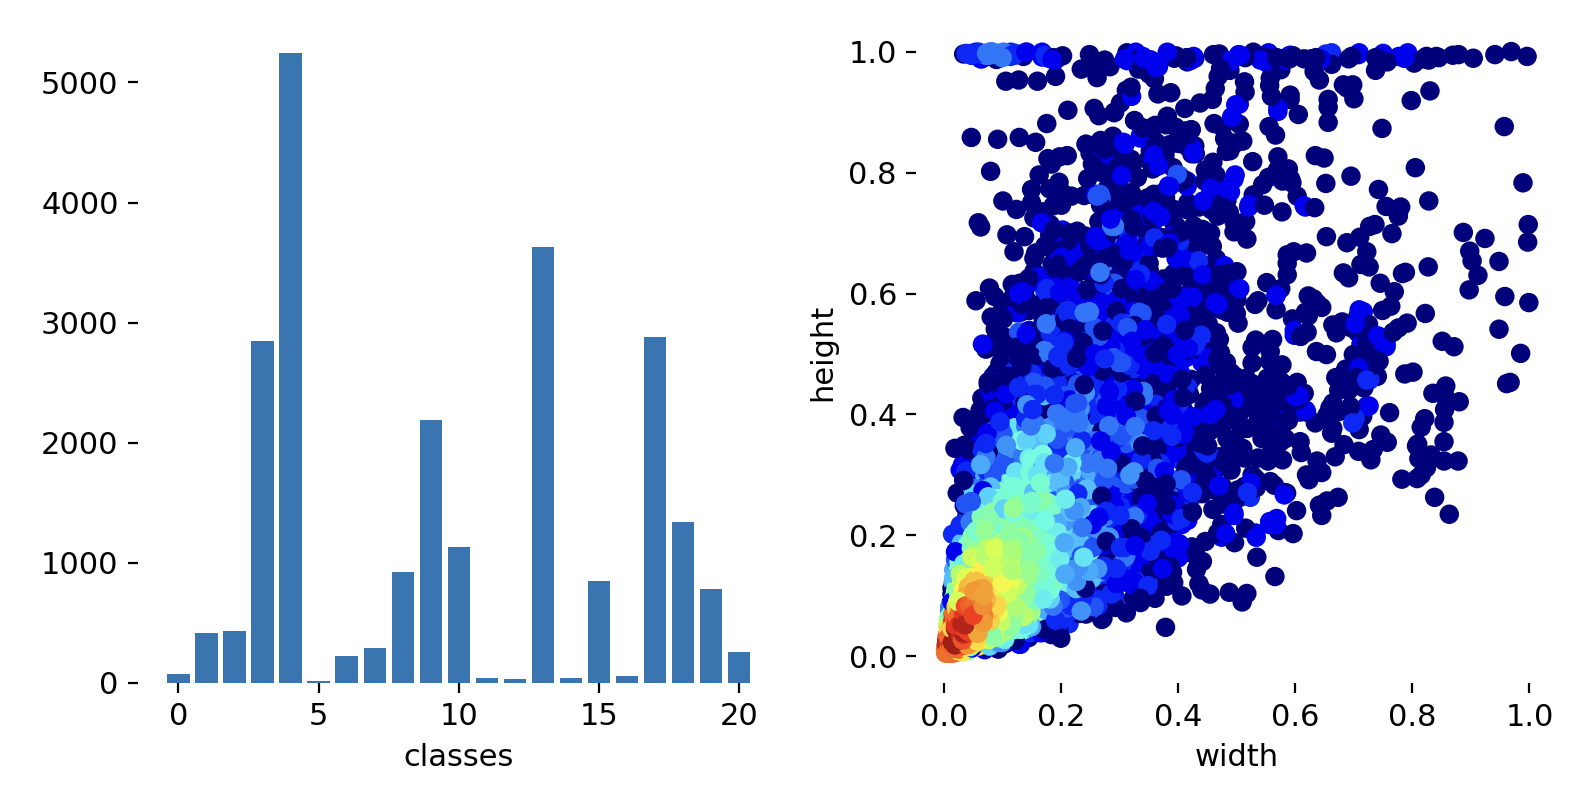
\includegraphics[max width=\textwidth]{images/ours/dhaka-ai+idd.png}
   \caption[Class Distribution of Dhaka AI+IDD dataset]{Class Distribution of Dhaka AI+IDD dataset}
    \label{fig:dhakaai_dataset}
\end{figure}

\subsubsection{List of Classes}
Our datasets contains 21 classes where some classes don't have much data compared to other classes. 

Here buses and cars have the highest number of data compared to others. For this accuracy of detecting other classes became difficult. We can reduce this by gathering more data but it is a hard job. We can also train models with only a few classes which will increase the accuracy rate of the model but we will lose the ability to detect other vehicles.


\begin{multicols}{2}
\begin{enumerate}
\item Ambulance
\item Auto Rickshaw
\item Bicycle
\item Bus
\item Car
\item Garbage Van
\item Human Hauler
\item Minibus
\item Minivan
\item Motorbike
\item Pickup
\item Army Vehicle
\item Police Car
\item Rickshaw
\item Scooter
\item SUV
\item Taxi
\item Three Wheelers (CNG)
\item Truck
\item Van
\item Wheelbarrow
\end{enumerate}
\end{multicols}

Above some of the classes have very low data like Wheelbarrow, Ambulance Garbage van etc. We tested our model by removing these classes and it gave good results but remove the ability to detect those classes.  
\newpage



